% Options for packages loaded elsewhere
\PassOptionsToPackage{unicode}{hyperref}
\PassOptionsToPackage{hyphens}{url}
\PassOptionsToPackage{dvipsnames,svgnames,x11names}{xcolor}
%
\documentclass[
  letterpaper,
  DIV=11,
  numbers=noendperiod]{scrartcl}

\usepackage{amsmath,amssymb}
\usepackage{lmodern}
\usepackage{iftex}
\ifPDFTeX
  \usepackage[T1]{fontenc}
  \usepackage[utf8]{inputenc}
  \usepackage{textcomp} % provide euro and other symbols
\else % if luatex or xetex
  \usepackage{unicode-math}
  \defaultfontfeatures{Scale=MatchLowercase}
  \defaultfontfeatures[\rmfamily]{Ligatures=TeX,Scale=1}
\fi
% Use upquote if available, for straight quotes in verbatim environments
\IfFileExists{upquote.sty}{\usepackage{upquote}}{}
\IfFileExists{microtype.sty}{% use microtype if available
  \usepackage[]{microtype}
  \UseMicrotypeSet[protrusion]{basicmath} % disable protrusion for tt fonts
}{}
\makeatletter
\@ifundefined{KOMAClassName}{% if non-KOMA class
  \IfFileExists{parskip.sty}{%
    \usepackage{parskip}
  }{% else
    \setlength{\parindent}{0pt}
    \setlength{\parskip}{6pt plus 2pt minus 1pt}}
}{% if KOMA class
  \KOMAoptions{parskip=half}}
\makeatother
\usepackage{xcolor}
\setlength{\emergencystretch}{3em} % prevent overfull lines
\setcounter{secnumdepth}{5}
% Make \paragraph and \subparagraph free-standing
\ifx\paragraph\undefined\else
  \let\oldparagraph\paragraph
  \renewcommand{\paragraph}[1]{\oldparagraph{#1}\mbox{}}
\fi
\ifx\subparagraph\undefined\else
  \let\oldsubparagraph\subparagraph
  \renewcommand{\subparagraph}[1]{\oldsubparagraph{#1}\mbox{}}
\fi


\providecommand{\tightlist}{%
  \setlength{\itemsep}{0pt}\setlength{\parskip}{0pt}}\usepackage{longtable,booktabs,array}
\usepackage{calc} % for calculating minipage widths
% Correct order of tables after \paragraph or \subparagraph
\usepackage{etoolbox}
\makeatletter
\patchcmd\longtable{\par}{\if@noskipsec\mbox{}\fi\par}{}{}
\makeatother
% Allow footnotes in longtable head/foot
\IfFileExists{footnotehyper.sty}{\usepackage{footnotehyper}}{\usepackage{footnote}}
\makesavenoteenv{longtable}
\usepackage{graphicx}
\makeatletter
\def\maxwidth{\ifdim\Gin@nat@width>\linewidth\linewidth\else\Gin@nat@width\fi}
\def\maxheight{\ifdim\Gin@nat@height>\textheight\textheight\else\Gin@nat@height\fi}
\makeatother
% Scale images if necessary, so that they will not overflow the page
% margins by default, and it is still possible to overwrite the defaults
% using explicit options in \includegraphics[width, height, ...]{}
\setkeys{Gin}{width=\maxwidth,height=\maxheight,keepaspectratio}
% Set default figure placement to htbp
\makeatletter
\def\fps@figure{htbp}
\makeatother
\newlength{\cslhangindent}
\setlength{\cslhangindent}{1.5em}
\newlength{\csllabelwidth}
\setlength{\csllabelwidth}{3em}
\newlength{\cslentryspacingunit} % times entry-spacing
\setlength{\cslentryspacingunit}{\parskip}
\newenvironment{CSLReferences}[2] % #1 hanging-ident, #2 entry spacing
 {% don't indent paragraphs
  \setlength{\parindent}{0pt}
  % turn on hanging indent if param 1 is 1
  \ifodd #1
  \let\oldpar\par
  \def\par{\hangindent=\cslhangindent\oldpar}
  \fi
  % set entry spacing
  \setlength{\parskip}{#2\cslentryspacingunit}
 }%
 {}
\usepackage{calc}
\newcommand{\CSLBlock}[1]{#1\hfill\break}
\newcommand{\CSLLeftMargin}[1]{\parbox[t]{\csllabelwidth}{#1}}
\newcommand{\CSLRightInline}[1]{\parbox[t]{\linewidth - \csllabelwidth}{#1}\break}
\newcommand{\CSLIndent}[1]{\hspace{\cslhangindent}#1}

\usepackage{booktabs}
\usepackage{longtable}
\usepackage{array}
\usepackage{multirow}
\usepackage{wrapfig}
\usepackage{float}
\usepackage{colortbl}
\usepackage{pdflscape}
\usepackage{tabu}
\usepackage{threeparttable}
\usepackage{threeparttablex}
\usepackage[normalem]{ulem}
\usepackage{makecell}
\usepackage{xcolor}
\KOMAoption{captions}{tableheading}
\makeatletter
\makeatother
\makeatletter
\makeatother
\makeatletter
\@ifpackageloaded{caption}{}{\usepackage{caption}}
\AtBeginDocument{%
\ifdefined\contentsname
  \renewcommand*\contentsname{Table of contents}
\else
  \newcommand\contentsname{Table of contents}
\fi
\ifdefined\listfigurename
  \renewcommand*\listfigurename{List of Figures}
\else
  \newcommand\listfigurename{List of Figures}
\fi
\ifdefined\listtablename
  \renewcommand*\listtablename{List of Tables}
\else
  \newcommand\listtablename{List of Tables}
\fi
\ifdefined\figurename
  \renewcommand*\figurename{Figure}
\else
  \newcommand\figurename{Figure}
\fi
\ifdefined\tablename
  \renewcommand*\tablename{Table}
\else
  \newcommand\tablename{Table}
\fi
}
\@ifpackageloaded{float}{}{\usepackage{float}}
\floatstyle{ruled}
\@ifundefined{c@chapter}{\newfloat{codelisting}{h}{lop}}{\newfloat{codelisting}{h}{lop}[chapter]}
\floatname{codelisting}{Listing}
\newcommand*\listoflistings{\listof{codelisting}{List of Listings}}
\makeatother
\makeatletter
\@ifpackageloaded{caption}{}{\usepackage{caption}}
\@ifpackageloaded{subcaption}{}{\usepackage{subcaption}}
\makeatother
\makeatletter
\@ifpackageloaded{tcolorbox}{}{\usepackage[many]{tcolorbox}}
\makeatother
\makeatletter
\@ifundefined{shadecolor}{\definecolor{shadecolor}{rgb}{.97, .97, .97}}
\makeatother
\makeatletter
\makeatother
\ifLuaTeX
  \usepackage{selnolig}  % disable illegal ligatures
\fi
\IfFileExists{bookmark.sty}{\usepackage{bookmark}}{\usepackage{hyperref}}
\IfFileExists{xurl.sty}{\usepackage{xurl}}{} % add URL line breaks if available
\urlstyle{same} % disable monospaced font for URLs
\hypersetup{
  pdftitle={Exploring Relationships between Demographic Characteristics, Health, Finances, Living Arrangements, and Happiness: An Analysis of the General Social Survey (GSS) Data from 1972 to 2012},
  pdfauthor={SHAOHAN CHANG},
  colorlinks=true,
  linkcolor={blue},
  filecolor={Maroon},
  citecolor={Blue},
  urlcolor={Blue},
  pdfcreator={LaTeX via pandoc}}

\title{Exploring Relationships between Demographic Characteristics,
Health, Finances, Living Arrangements, and Happiness: An Analysis of the
General Social Survey (GSS) Data from 1972 to 2012\thanks{Code and data
are available at: https://github.com/lucas11333/Factor\_of\_Wellbeing}}
\author{SHAOHAN CHANG}
\date{28 March 2023}

\begin{document}
\maketitle
\begin{abstract}
This paper presents an analysis of a subset of the General Social Survey
(GSS) data from the year 1972, which includes information on
individuals' demographic characteristics, health, finances, living
arrangements, and subjective well-being. The study aimed to explore
various aspects of individuals' lives during the early 1970s in the
United States, such as social stratification, gender roles, family
dynamics, health disparities, and subjective well-being.The dataset
consists of 5 observations and 10 variables, including year, age, sex,
babies, divorce, health, finance\_satisfied, living\_area, and happy.
The study used graphical representation to analyze the relationships
between different variables in the dataset and individuals' level of
happiness. The results of the analysis suggest that there is a positive
relationship between people's satisfaction with their current financial
situation, their self-rated health, and their level of happiness in
life. Additionally, being divorced may have a slight impact on one's
level of happiness in life, with a small proportion of individuals
feeling not too happy. Moreover, the study found that people's level of
education is positively associated with their level of happiness in
life, as people's education level increases, their level of happiness
also gradually increases.Overall, this study provides valuable insights
into various aspects of individuals' lives during the early 1970s in the
United States. The findings can be useful for researchers and students
interested in exploring topics such as social stratification, gender
roles, family dynamics, health disparities, and subjective well-being.
The study highlights the importance of considering different factors
that can influence individuals' level of happiness and well-being, such
as their financial situation, health status, and level of education.
Further research could investigate more recent data from the GSS to
examine changes in these relationships over time.
\end{abstract}
\ifdefined\Shaded\renewenvironment{Shaded}{\begin{tcolorbox}[frame hidden, breakable, borderline west={3pt}{0pt}{shadecolor}, sharp corners, enhanced, interior hidden, boxrule=0pt]}{\end{tcolorbox}}\fi

\hypertarget{introduction}{%
\section{Introduction}\label{introduction}}

Surveys are a common method for collecting data on individuals'
attitudes, behaviors, and experiences in social science research. One
such survey is the General Social Survey (GSS), which has been conducted
in the United States since 1972 to 2012. This data set is a subset of
the GSS data from the year 1972, which includes information on
individuals' demographic characteristics, health, finances, living
arrangements, and subjective well-being. While this is a relatively
small data set, it provides a glimpse into the lives of individuals in
the United States during a particular period in time.This paper aims to
explore various aspects of individuals' lives during the early 1970s in
the United States using the GSS data set. The variables in this data set
are diverse and reflect a range of aspects of individuals' lives. For
instance, the variables on babies and divorce provide information on
individuals' family structures, while the variables on health and
finance satisfaction offer insights into their well-being and financial
stability (Vlaev 2014). The data set also includes variables on
individuals' living arrangements and their subjective well-being,
providing a glimpse into their social context and overall happiness.

The paper presents a comprehensive analysis of the relationships between
different variables in the data set and individuals' level of happiness.
The analysis includes a graphical representation of the relationship
between the number of children and happiness in the family, individuals'
self-rated health and their self-rated level of happiness, people's
satisfaction with their financial situation and their happiness, the
level of happiness in life for individuals in two different states:
divorced or married, and the relationship between people's level of
education and their level of happiness in life.The results of the
analysis suggest that there is a positive relationship between people's
satisfaction with their current financial situation, their self-rated
health, and their level of happiness in life (RSiahpush 2008). The
analysis also indicates that being divorced may have a slight impact on
one's level of happiness in life, with a small proportion of individuals
feeling ``not too happy.'' Additionally, as people's education level
increases, their level of happiness also gradually increases.

Overall, this paper provides valuable insights into various aspects of
individuals' lives during the early 1970s in the United States. The
findings can be useful for researchers and students interested in
exploring topics such as social stratification, gender roles, family
dynamics, health disparities, and subjective well-being.

\hypertarget{methodology}{%
\subsection{Methodology}\label{methodology}}

This study will combine data sources, including surveys and academic
literature. The collected data will be analyzed to determine the trends
and changes in public attitudes towards sexual morality over time (1972
to 2012). The study will also examine differences in attitudes between
men and women, as well as work attitudes, and the relationship between
education levels and happiness in daily life.

\hypertarget{data-resource}{%
\section{Data Resource}\label{data-resource}}

Used some R language packages, such as tidyverse (Wickham et al. 2019),
dplyr (Wickham et al. 2023), janitor (Firke 2023) , knitr (Xie 2014),
here (Müller 2020), haven (Wickham, Miller, and Smith 2022), ggplot
(Wickham 2016) , kableExtra (Zhu 2021) to assist in data analysis, and
the data from General Social Survey ({``GSS General Social Survey''}
2023).

\hypertarget{sec-data}{%
\subsection{Data}\label{sec-data}}

After cleaning the data and selecting the main variables, the following
table shows the first five rows of data and their corresponding
parameters.The following data section provides a more detailed
explanation of the selected variables for the data.

This data-set contains information on various personal and demographic
characteristics of individuals, collected between the years 1972 and
2012. The data-set includes variables such as age, sex, number of
babies, divorce status, self-reported health status, financial
satisfaction, living area, and level of happiness. The data-set can be
used to study the relationships between these variables and to gain
insights into factors that may influence an individual's overall life
satisfaction.

\begin{table}

\caption{Table of Happy by Various Variables}
\centering
\begin{tabular}[t]{r|l|l|l|l|l|l|l}
\hline
year & age & sex & babies & divorce & health & finance\_satified & living\_area\\
\hline
1972 & 70 & male & 0 & no & fair & more or less satisfied & large city\\
\hline
1972 & 48 & female & 0 & no & excellent & pretty well satisfied & large city\\
\hline
1972 & 27 & female & 0 & no & good & not satisfied at all & large city\\
\hline
1972 & 61 & female & 0 & no & good & pretty well satisfied & unknown\\
\hline
1972 & 30 & female & 2 & no & fair & not satisfied at all & unknown\\
\hline
\end{tabular}
\end{table}

\begin{table}
\centering
\begin{tabular}{l|l}
\hline
happy & degree\\
\hline
not too happy & less than high school\\
\hline
happy & high school\\
\hline
not too happy & bachelor's\\
\hline
happy & high school\\
\hline
happy & high school\\
\hline
\end{tabular}
\end{table}

\begin{itemize}
\tightlist
\item
  year: This variable indicates the year in which the data was
  collected. In this data-set, all the observations are from the year
  1972 to 2012.
\item
  age: This variable indicates the age of the individual at the time the
  data was collected. It is a continuous variable measured in years.
\item
  sex: This variable indicates the biological sex of the individual. It
  is a categorical variable with two levels: male and female.
\item
  babies: This variable indicates the number of babies the individual
  had at the time the data was collected. It is a categorical variable
  with different levels, depending on the number of babies: 0, 1, 2, 3,
  4, or 5+.
\item
  divorce: This variable indicates whether or not the individual had
  ever been divorced at the time the data was collected. It is a
  categorical variable with two levels: yes and no.
\item
  health: This variable indicates the self-reported health status of the
  individual at the time the data was collected. It is a categorical
  variable with different levels, depending on the health status:
  excellent, good, fair, or poor.
\item
  finance\_satisfied: This variable indicates the individual's level of
  satisfaction with their current financial situation. It is a
  categorical variable with different levels of satisfaction: very
  satisfied, more or less satisfied, not very satisfied, and not at all
  satisfied.
\item
  living\_area: This variable indicates the type of living area in which
  the individual resided at the time the data was collected. It is a
  categorical variable with different levels: large city, small city,
  suburban, and rural.
\item
  happy: This variable indicates the individual's level of happiness or
  life satisfaction. It is a categorical variable with different levels
  of happiness: very happy, pretty happy, not too happy, and not at all
  happy.
\end{itemize}

In Figure~\ref{fig-one}, this chart shows the number of people who are
very happy, not too happy, and happy. Overall, the data indicates that
the largest number of people are happy, with approximately 15,000
individuals falling into this category. On the other hand, the smallest
number of people are not too happy, with significantly fewer individuals
in this category compared to the other two variables. In summary, the
data suggests that the number of unhappy individuals is a relatively
small group.

\begin{figure}

{\centering 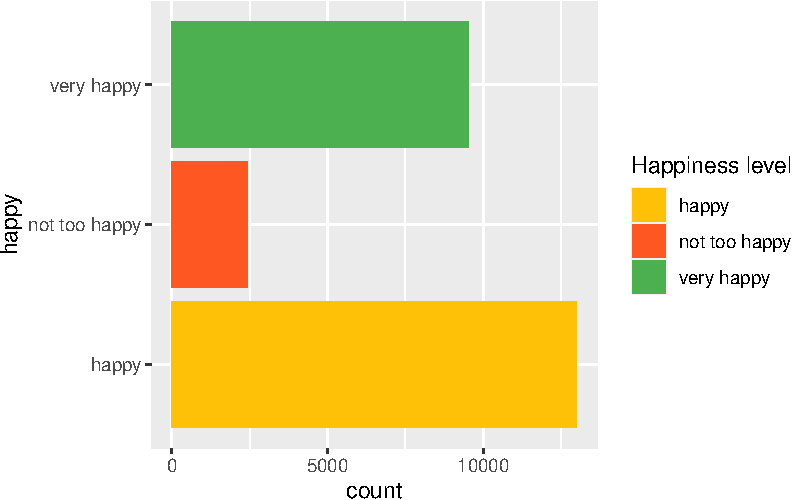
\includegraphics{paper_files/figure-pdf/fig-one-1.pdf}

}

\caption{\label{fig-one}Couning of Happiness}

\end{figure}

\hypertarget{baby}{%
\subsubsection{Baby}\label{baby}}

In Figure~\ref{fig-two}, through the graph showing the relationship
between the number of children and happiness in the family, it is
obvious that when people have no children, the largest number of `very
happy', `pretty happy', and `not too happy' are shown. Although The
preliminary judgment is that the number of people who are happy without
children is the largest. But among the data, the data collected without
children is the most. In order to ensure the accuracy of the data, it is
necessary to further analyze the proportion of the number of children in
the family for the next part of the analysis.

\begin{figure}

{\centering 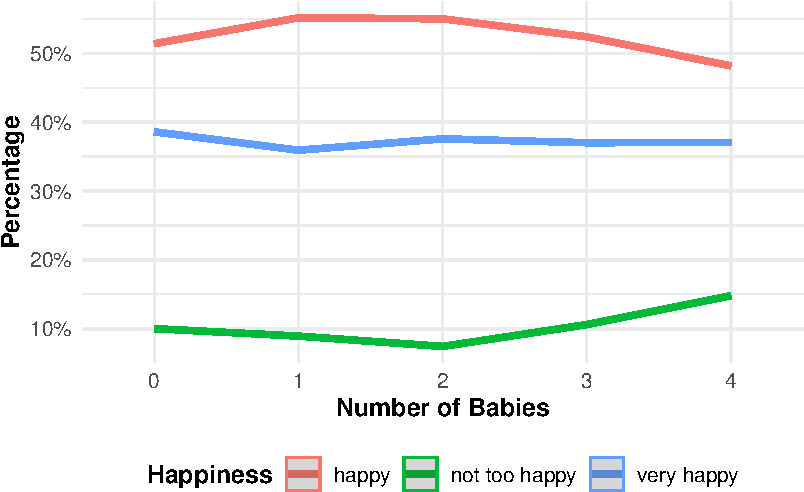
\includegraphics{paper_files/figure-pdf/fig-two-1.pdf}

}

\caption{\label{fig-two}Relationship between Number of Babies and
Happiness}

\end{figure}

In Figure~\ref{fig-three}, which to provide a more detailed and
comprehensive view of the data, the chart displays an analysis and
visualization of the number of children had each year from 1972 to 2012,
in relation to the level of happiness. In regards to the variable ``not
too happy,'' the proportion of individuals who reported feeling unhappy
was relatively high in 1974, 1985, 1993, 2004, 2006, and 2008. On the
other hand, in regards to the variable ``happy,'' the percentage of
individuals reporting feeling happy was relatively high in 1973, 1977,
1994, 2006, and 2012.

\begin{figure}

{\centering 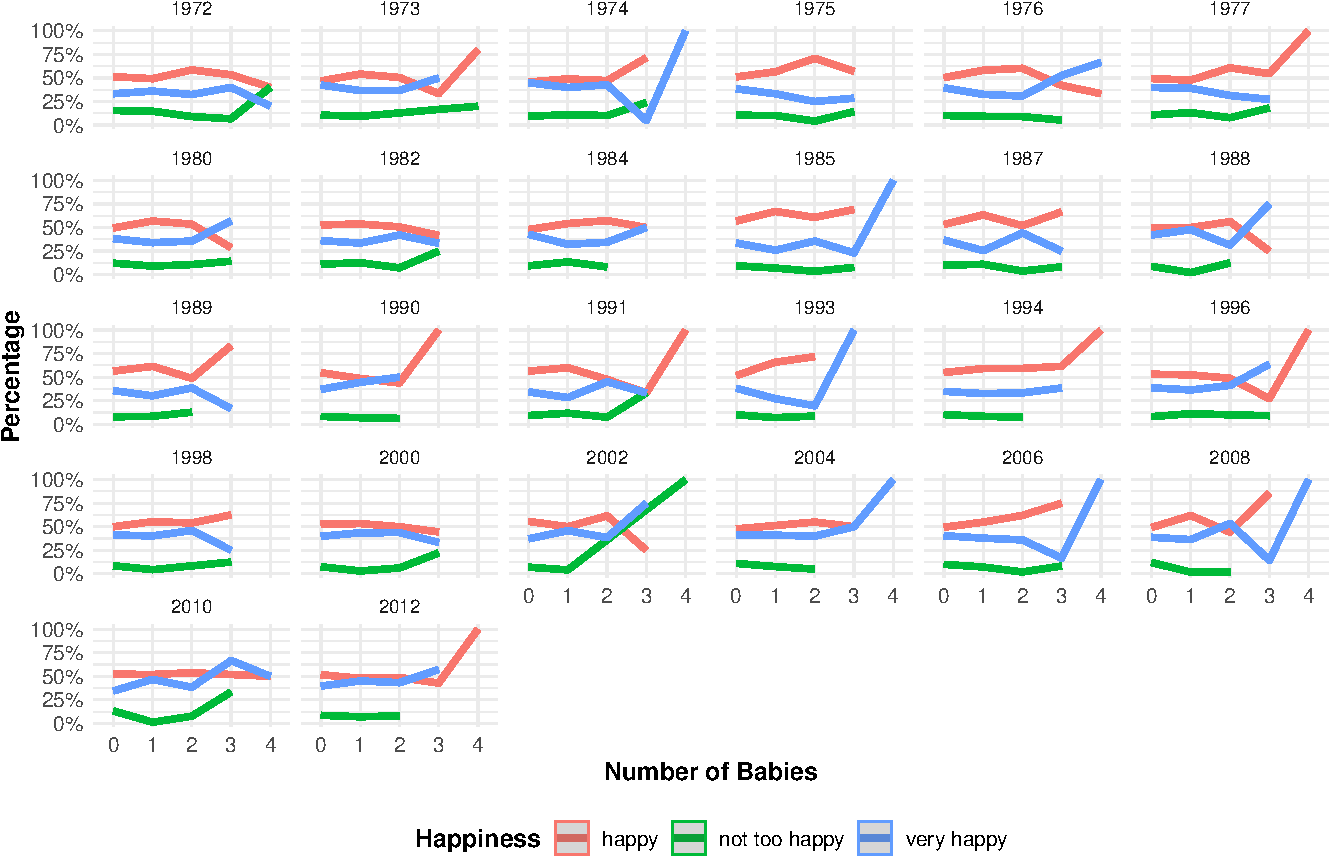
\includegraphics{paper_files/figure-pdf/fig-three-1.pdf}

}

\caption{\label{fig-three}Relationship between Number of Babies and
Happiness by Year}

\end{figure}

\hypertarget{health}{%
\subsubsection{Health}\label{health}}

In Figure~\ref{fig-four}, which represents the relationship between
participants' self-rated health and their self-rated level of happiness.
The chart shows that the proportion of participants who rated themselves
as ``very happy'' was the highest among those who rated their health as
``excellent''. On the other hand, the proportion of participants who
rated themselves as ``not too happy'' was the lowest among those who
rated their health as ``poor''.From the overall trend, it can be
inferred that the higher the participants' self-rated health, the higher
their self-rated level of satisfaction with life.

\begin{figure}

{\centering 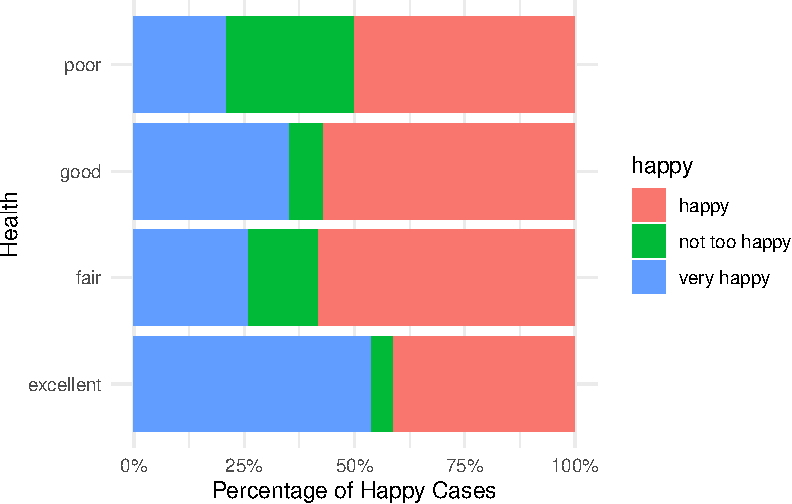
\includegraphics{paper_files/figure-pdf/fig-four-1.pdf}

}

\caption{\label{fig-four}Relationship between Health and Happiness}

\end{figure}

In Figure~\ref{fig-five}, which spanning from 1970 to 2010, illustrates
the relationship between participants' self-reported happiness levels
and their health states. It is evident that when participants rated
their health as `poor', the proportion of those who identified as `very
happy' was notably lower compared to other health states. On the other
hand, when participants reported their health as `excellent' or `good',
the number of `very happy' responses regarding their life satisfaction
increased significantly. In summary, this chart suggests a positive
correlation between people's health and their happiness in life.

\begin{figure}

{\centering 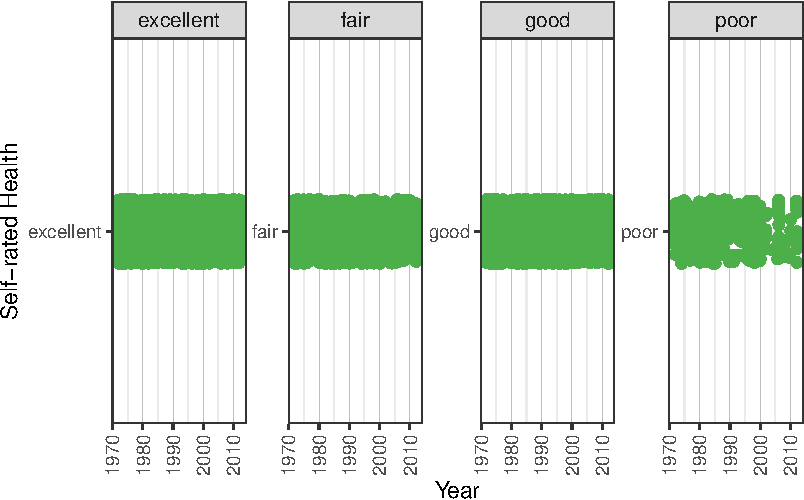
\includegraphics{paper_files/figure-pdf/fig-five-1.pdf}

}

\caption{\label{fig-five}Relationship between Health and ``Very Happy''
With Year}

\end{figure}

\hypertarget{financial-satisfaction}{%
\subsubsection{Financial Satisfaction}\label{financial-satisfaction}}

In Figure~\ref{fig-six}, the graph depicts the relationship between
people's satisfaction with their financial situation and their
happiness.It is clear that when people are not very satisfied with their
current finances, the proportion of unhappy people in their lives is the
highest. On the other hand, when people are very satisfied with their
finances, the proportion of happy people in their lives is the highest,
and the proportion of unhappy people is also the lowest. Therefore, it
can be concluded that there is a positive relationship between people's
satisfaction with their current financial situation and their level of
happiness in life.

\begin{figure}

{\centering 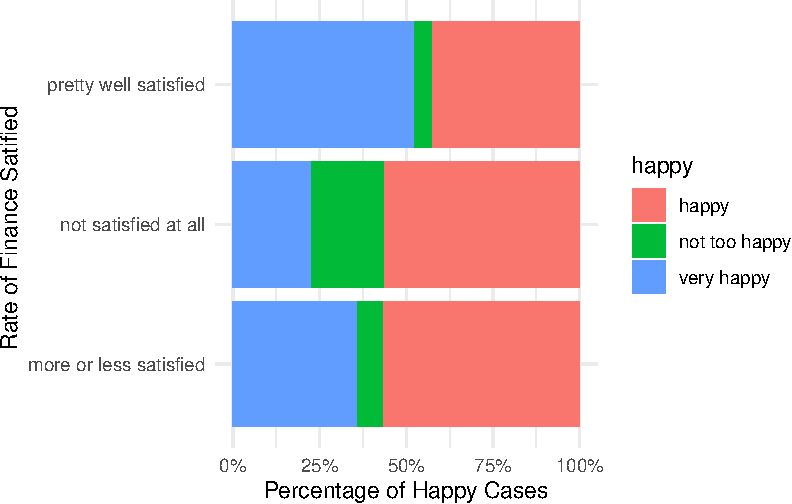
\includegraphics{paper_files/figure-pdf/fig-six-1.pdf}

}

\caption{\label{fig-six}Relationship between Happiness and finance
satified}

\end{figure}

\hypertarget{divorce}{%
\subsubsection{Divorce}\label{divorce}}

In Figure~\ref{fig-seven}, the graph represents the level of happiness
in life for individuals in two different states: divorced or married.
The graph shows that the levels of happiness in both marital states are
almost similar. However, the proportion of people who feel ``not too
happy'' in their lives is slightly higher among the divorced group than
among the married group. In conclusion, being divorced may have a slight
impact on one's level of happiness in life, with a small proportion of
individuals feeling ``not too happy.''

\begin{figure}

{\centering 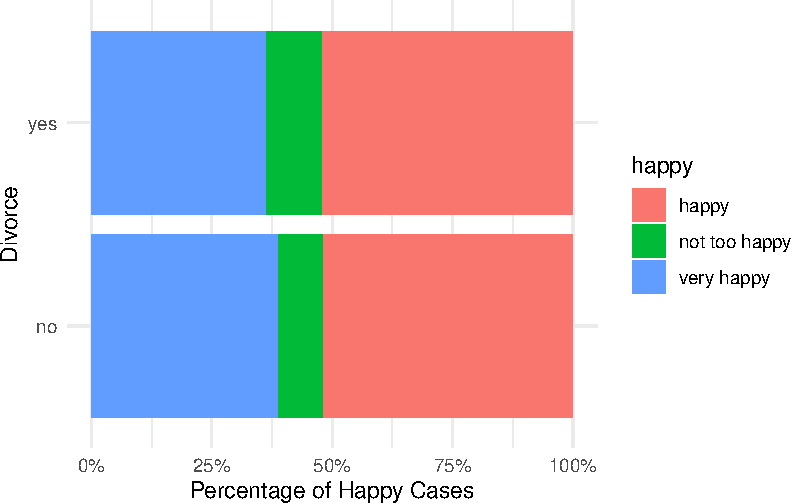
\includegraphics{paper_files/figure-pdf/fig-seven-1.pdf}

}

\caption{\label{fig-seven}Relationship between Happiness and Divorce}

\end{figure}

In Figure~\ref{fig-eight}, which based on the analysis of the charts, it
appears that for the years 1972, 1975, 1982, 1990, 1996, 2002, and 2010,
individuals who reported being divorced also reported a higher
percentage of happy responses. On the other hand, for the years 1976,
1980, 1984, 1987, 1989, and 2006, individuals who reported being married
reported a higher percentage of happy responses. Additionally, the
percentage of individuals who reported ``not too happy'' was
significantly higher for individuals who reported being divorced than
for those who reported being married in the years 1973, 1984, 1987,
1990, 1991, 1993, 2008, and 2012.

\begin{figure}

{\centering 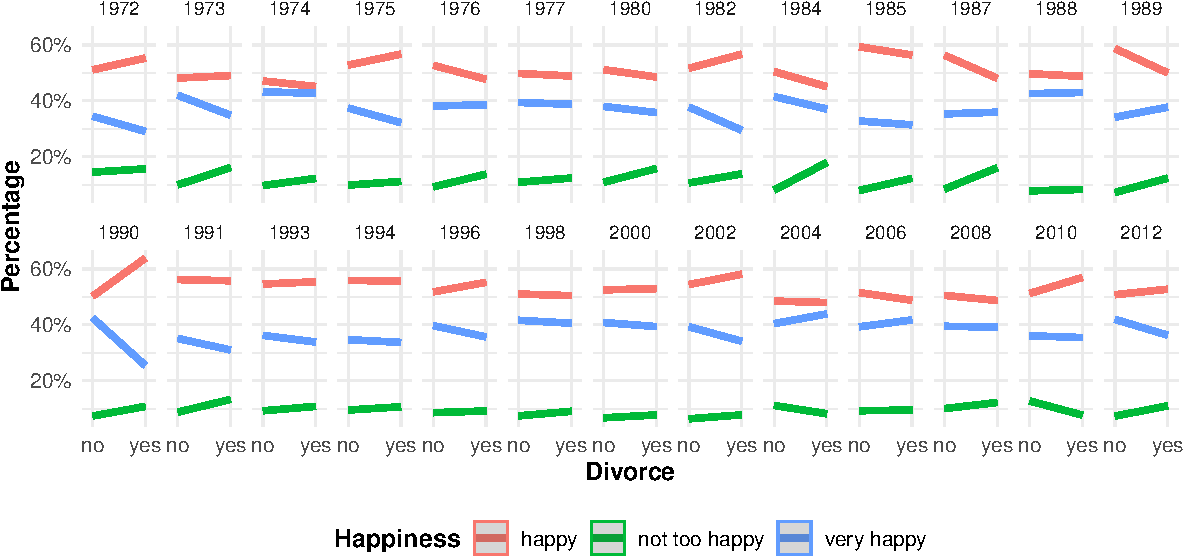
\includegraphics{paper_files/figure-pdf/fig-eight-1.pdf}

}

\caption{\label{fig-eight}Relationship between Divorce and Happiness by
Year}

\end{figure}

\hypertarget{degree}{%
\subsubsection{Degree}\label{degree}}

In Figure~\ref{fig-nine}, which shows that there is a certain
relationship between people's level of education and their level of
happiness in life. From the graph, it can be observed that the
proportion of people who feel ``not too happy'' is the highest among
those with education levels lower than high school. However, the
proportion of unhappy individuals is the lowest among those with
bachelor's and graduate degrees, suggesting that as people's education
level increases, their level of happiness also gradually increases.

\begin{figure}

{\centering 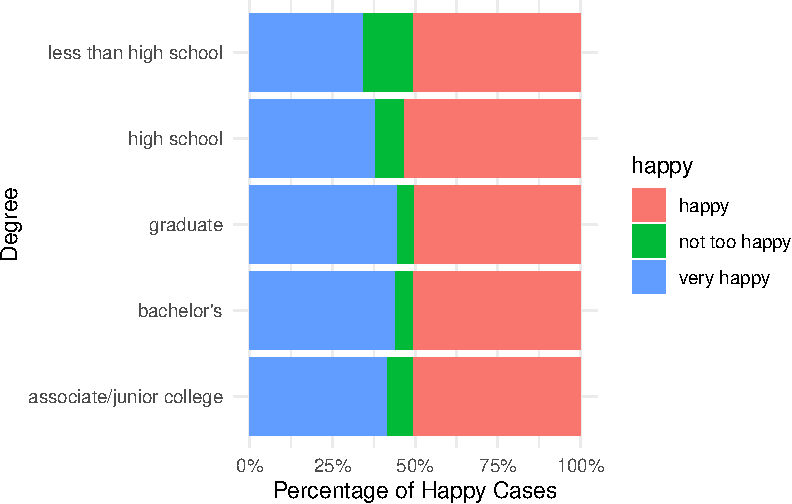
\includegraphics{paper_files/figure-pdf/fig-nine-1.pdf}

}

\caption{\label{fig-nine}Relationship between Happiness and Degree}

\end{figure}

\hypertarget{model}{%
\section{Model}\label{model}}

\begin{verbatim}

Call:
lm(formula = happy_score ~ age + degree + finance_satified + 
    health + divorce, data = data)

Coefficients:
                          (Intercept)                                    age  
                             4.951478                              -0.002144  
                     degreebachelor's                         degreegraduate  
                             0.028053                               0.026886  
                    degreehigh school            degreeless than high school  
                            -0.005915                              -0.106730  
 finance_satifiednot satisfied at all  finance_satifiedpretty well satisfied  
                            -0.471882                               0.087194  
                           healthfair                             healthgood  
                            -0.315050                              -0.063929  
                           healthpoor                             divorceyes  
                            -0.747780                              -0.018373  
\end{verbatim}

\hypertarget{summary}{%
\section{summary}\label{summary}}

\hypertarget{table-of-relationship-between-number-of-children-and-happiness-in-the-family.}{%
\subsection{Table of Relationship between Number of Children and
Happiness in the
Family.}\label{table-of-relationship-between-number-of-children-and-happiness-in-the-family.}}

In the table two, which appears to be presenting data on the happiness
levels of babies, as rated by some measure or criteria, at different
ages from 0 to 4 years old. The three categories of happiness levels are
``not too happy,'' ``happy,'' and ``very happy.'' Looking at the data
for 4-year-old, we can see that 48.15\% of them were rated as ``not too
happy,'' 14.81\% as ``very happy,'' and the remaining 37.04\% as simply
``happy.'' This suggests that the majority of 4-year-old were not rated
as particularly happy, with less than half of them falling into the
happy or very happy categories.

\begin{table}

\caption{Table of Happy by Various Variables}
\centering
\begin{tabular}[t]{l|r|r|r}
\hline
babies & happy & not too happy & very happy\\
\hline
0 & 51.37 & 10.04 & 38.59\\
\hline
1 & 55.13 & 8.96 & 35.91\\
\hline
2 & 54.97 & 7.46 & 37.57\\
\hline
3 & 52.36 & 10.63 & 37.01\\
\hline
4 & 48.15 & 14.81 & 37.04\\
\hline
\end{tabular}
\end{table}

\hypertarget{table-of-health-and-happiness-in-the-family}{%
\subsection{Table of Health and Happiness in the
Family}\label{table-of-health-and-happiness-in-the-family}}

In table three, which appears to be presenting data on the relationship
between the health and happiness levels of families, based on some
measure or criteria. The three categories of happiness levels are ``not
too happy,'' ``happy,'' and ``very happy,'' while the four categories of
health are ``excellent,'' ``fair,'' ``good,'' and ``poor.'' Looking at
the data, we can see that families who rated their health as
``excellent'' had the highest proportion of respondents who reported
being ``very happy,'' at 53.70\%, and the lowest proportion of those who
were ``not too happy,'' at only 4.94\%. In contrast, families who rated
their health as ``fair'' had the highest proportion of respondents who
were ``not too happy,'' at 15.92\%, and the lowest proportion of those
who were ``very happy,'' at only 25.81\%.

\begin{table}

\caption{Table of Health and Happiness in the Family}
\centering
\begin{tabular}[t]{l|r|r|r}
\hline
health & happy & not too happy & very happy\\
\hline
excellent & 41.37 & 4.94 & 53.70\\
\hline
fair & 58.27 & 15.92 & 25.81\\
\hline
good & 57.14 & 7.76 & 35.10\\
\hline
poor & 50.14 & 29.09 & 20.77\\
\hline
\end{tabular}
\end{table}

\hypertarget{table-of-financial-satisfaction-and-happiness-in-the-family}{%
\subsection{Table of Financial Satisfaction and Happiness in the
Family}\label{table-of-financial-satisfaction-and-happiness-in-the-family}}

In table four, which appears that the table is presenting data on the
relationship between financial satisfaction and happiness levels in
families, based on some measure or criteria. The three categories of
happiness levels are ``not too happy,'' ``happy,'' and ``very happy,''
while the three categories of financial satisfaction are ``more or less
satisfied,'' ``not satisfied at all,'' and ``pretty well satisfied.''
Looking at the data, we can see that families who reported being
``pretty well satisfied'' with their finances had the highest proportion
of respondents who were ``very happy,'' at 52.0\%, and the lowest
proportion of those who were ``not too happy,'' at only 5.24\%. On the
other hand, families who reported being ``not satisfied at all'' with
their finances had the highest proportion of respondents who were ``not
too happy,'' at 20.92\%, and the lowest proportion of those who were
``very happy,'' at only 22.5\%.

\begin{table}

\caption{Table of Financial Satisfaction and Happiness in the Family}
\centering
\begin{tabular}[t]{l|r|r|r}
\hline
finance\_satified & happy & not too happy & very happy\\
\hline
more or less satisfied & 56.76 & 7.74 & 35.5\\
\hline
not satisfied at all & 56.59 & 20.92 & 22.5\\
\hline
pretty well satisfied & 42.75 & 5.24 & 52.0\\
\hline
\end{tabular}
\end{table}

In table five, which appears to be presenting data on the relationship
between divorce and happiness levels in families, based on some measure
or criteria. The three categories of happiness levels are ``not too
happy,'' ``happy,'' and ``very happy,'' while the two categories of
divorce are ``no'' and ``yes.'' Looking at the data, we can see that
there are only small differences in the proportions of families who
reported being ``happy'' or ``not too happy'' depending on whether or
not they had experienced divorce. Specifically, families who reported
``no'' to divorce had a slightly higher proportion of respondents who
were ``very happy,'' at 38.61\%, compared to those who reported ``yes''
to divorce, at 36.24\%. However, families who reported ``yes'' to
divorce had a slightly higher proportion of respondents who were ``not
too happy,'' at 11.53\%, compared to those who reported ``no'' to
divorce, at 9.29\%.

\begin{table}

\caption{Table of Divorce and Happiness in the Family}
\centering
\begin{tabular}[t]{l|r|r|r}
\hline
divorce & happy & not too happy & very happy\\
\hline
no & 52.10 & 9.29 & 38.61\\
\hline
yes & 52.23 & 11.53 & 36.24\\
\hline
\end{tabular}
\end{table}

In table six, which appears to be presenting data on the relationship
between educational attainment and happiness levels in families, based
on some measure or criteria. The three categories of happiness levels
are ``not too happy,'' ``happy,'' and ``very happy,'' while the
categories of educational attainment are ``associate/junior college,''
``bachelor's,'' ``graduate,'' ``high school,'' and ``less than high
school.'' Looking at the data, we can see that families with different
levels of educational attainment generally reported similar levels of
happiness. The proportions of respondents who reported being ``very
happy'' were similar across all levels of educational attainment,
ranging from 41.24\% for those with an associate/junior college degree
to 44.28\% for those with a graduate degree. The proportions of
respondents who reported being ``not too happy'' were also similar
across all levels of educational attainment, ranging from 5.26\% for
those with a graduate degree to 14.96\% for those with less than a high
school education.

\begin{table}

\caption{Table of Degree and Happiness in the Family}
\centering
\begin{tabular}[t]{l|r|r|r}
\hline
degree & happy & not too happy & very happy\\
\hline
associate/junior college & 50.85 & 7.91 & 41.24\\
\hline
bachelor's & 50.66 & 5.63 & 43.71\\
\hline
graduate & 50.47 & 5.26 & 44.28\\
\hline
high school & 53.48 & 8.86 & 37.66\\
\hline
less than high school & 50.90 & 14.96 & 34.13\\
\hline
\end{tabular}
\end{table}

\hypertarget{results}{%
\section{Results}\label{results}}

The analysis of the General Social Survey data-set from 1972 provides
insights into various aspects of individuals' lives in the United States
during that time period. The results suggest that several variables,
such as financial satisfaction, self-reported health status, and level
of education, have a positive relationship with individuals' level of
happiness.Regarding family dynamics, the analysis indicates that
individuals with no children reported the highest levels of happiness,
although the data set's limitations require further exploration of the
proportion of individuals with different numbers of children. Being
divorced may have a slight impact on one's level of happiness in life,
with a small proportion of individuals feeling ``not too happy''
compared to married individuals.

Furthermore, the analysis suggests that individuals' self-rated health
status has a positive relationship with their self-rated level of
happiness. The higher the participants' self-rated health, the higher
their self-rated level of satisfaction with life. Similarly, there is a
positive relationship between people's satisfaction with their current
financial situation and their level of happiness in life. The higher
people's satisfaction with their finances, the higher their level of
happiness.The analysis suggests that there is a certain relationship
between people's level of education and their level of happiness in
life. The proportion of people who feel ``not too happy'' is the highest
among those with education levels lower than high school. However, the
proportion of unhappy individuals is the lowest among those with
bachelor's and graduate degrees, suggesting that as people's education
level increases, their level of happiness also gradually increases.

Overall, these findings provide valuable insights into the factors that
may influence individuals' overall life satisfaction during the early
1970s in the United States. The results can be useful for researchers
and students interested in exploring topics such as social
stratification, gender roles, family dynamics, health disparities, and
subjective well-being.

\hypertarget{discussion}{%
\section{Discussion}\label{discussion}}

\hypertarget{factors-influencing-individuals-level-of-happiness}{%
\subsection{Factors influencing individuals' level of
happiness}\label{factors-influencing-individuals-level-of-happiness}}

The study's findings on the positive relationship between financial
satisfaction, health, and happiness underscore the importance of
financial stability and access to healthcare for overall well-being.
These findings have important implications for policymakers and
practitioners working to improve individuals' quality of life (Ory 1994)
. For example, policies aimed at increasing access to affordable
healthcare and financial assistance programs can help individuals
improve their financial stability and access to essential services,
ultimately contributing to overall well-being.

The study's results also suggest that education is an important factor
in individuals' overall well-being and happiness. As people's education
level increases, their level of happiness also gradually increases. This
highlights the need for policies and programs that support educational
attainment, particularly for disadvantaged populations (Rothstein 1994).
Such programs can include initiatives to improve access to education and
financial aid for those who may face barriers to education.

Overall, this study demonstrates the importance of considering various
factors that can influence individuals' well-being and happiness. By
understanding the complex relationships between different variables,
policymakers and practitioners can develop targeted interventions aimed
at improving individuals' quality of life. Additionally, the findings
can serve as a foundation for further research on the topic,
particularly in examining changes in these relationships over time.

\hypertarget{impact-of-divorce-on-individuals-happiness}{%
\subsection{Impact of divorce on individuals'
happiness}\label{impact-of-divorce-on-individuals-happiness}}

Divorce is a significant life event that can have profound effects on an
individual's overall well-being and happiness. The findings of this
study suggest that individuals who have experienced divorce may have
lower levels of happiness than those who are married or have never been
married. This could be due to a range of factors, including the loss of
social support and economic stability that often accompanies divorce
(Headey 1989).

One possible explanation for the association between divorce and
happiness is the impact of social support. Marriage provides a source of
emotional support, and individuals who divorce may experience a loss of
this support network. Furthermore, divorce can result in the breakdown
of extended family relationships, reducing the availability of social
support. This loss of social support could contribute to lower levels of
happiness and well-being. Economic factors may also play a role in the
relationship between divorce and happiness (Çakar 2020). Divorce can
result in significant financial upheaval, particularly for individuals
who were financially dependent on their partner. This financial
instability could contribute to lower levels of happiness and
well-being, as financial stress can be a significant source of anxiety
and depression.

Further research could explore the reasons behind the association
between divorce and happiness. Qualitative studies could be conducted to
explore the experiences of individuals who have gone through divorce and
how this event has affected their well-being. Longitudinal studies could
also be conducted to examine changes in individuals' happiness levels
before and after a divorce(Lucas 2003).

Overall, the findings of this study highlight the importance of
considering the impact of divorce on individuals' well-being and
happiness. Policies and interventions aimed at supporting individuals
going through divorce, such as access to counseling and financial
support, could help to mitigate the negative effects of this life event
and improve individuals' overall well-being.

\hypertarget{the-importance-of-historical-context-in-understanding-well-being}{%
\subsection{The importance of historical context in understanding
well-being}\label{the-importance-of-historical-context-in-understanding-well-being}}

The historical context of the early 1970s in the United States is
essential in understanding individuals' well-being during that period.
Societal norms, values, and attitudes during this time were different
from those of today, and these differences could have influenced
individuals' well-being. These social movements may have influenced
individuals' attitudes towards social stratification, gender roles, and
family dynamics, which, in turn, could have affected their well-being.

Understanding the historical context is also essential in developing
interventions that can address the unique challenges faced by
individuals during a particular period in time (Cooper 2005). For
example, the economic conditions during the early 1970s, such as high
inflation and high unemployment rates, could have affected individuals'
financial stability and, ultimately, their well-being. Interventions
that address these economic challenges may have had a significant impact
on individuals' well-being during this period.

Furthermore, the study's findings can be compared to more recent data to
examine changes in the relationships between different factors and
well-being over time (CBrunstein 1993). For example, the impact of
divorce on well-being may have changed over time, as societal attitudes
towards divorce have shifted. Comparing the study's findings to more
recent data can provide insights into how societal changes have
influenced individuals' well-being over time.Overall, the historical
context is essential in understanding individuals' well-being during a
particular period in time. The study's focus on the early 1970s in the
United States provides valuable insights into the factors that
influenced individuals' well-being during that period. These findings
can be used to develop interventions that address the unique challenges
faced by individuals during a particular historical context, as well as
to compare changes in the relationships between different factors and
well-being over time.

\hypertarget{impact-of-financial-stability-on-happiness}{%
\subsection{Impact of Financial Stability on
Happiness}\label{impact-of-financial-stability-on-happiness}}

As the analysis of the GSS dataset shows, there is a positive
correlation between individuals' satisfaction with their financial
situation and overall well-being, an important finding. This correlation
underscores the importance of U.S. financial stability in determining a
person's happiness in the early 1970s. In this discussion, we will
further explore the impact of these factors on individual well-being
during that time.

In the early 1970s, the United States was going through a period of
economic turmoil. One of the most important factors is the rapid rise in
inflation. The country faces a phenomenon known as ``stagflation,''
which is characterized by a stagnant economy, high inflation, and high
unemployment. This unusual economic situation is largely attributable to
the 1973 oil crisis, which caused a spike in oil prices and disrupted
the global economy (Barsky 2001). The rise in inflation during this
period has a direct impact on individuals' financial satisfaction. As
the cost of goods and services increases, people find it a challenge to
maintain their previous standard of living (Diener 2009). This is
further exacerbated by high unemployment, as many people struggle to
find stable employment.Analysis of the GSS dataset highlights the
importance of financial stability in determining individual well-being,
emphasizing the need for effective economic policies to ensure the
financial security and well-being of populations.

\hypertarget{the-role-of-education-in-happiness}{%
\subsection{The Role of Education in
Happiness}\label{the-role-of-education-in-happiness}}

The study found that as an individual's education level increased, their
level of happiness also gradually increased. This finding prompts a
discussion on the role of education in determining one's overall
happiness and well-being during the early 1970s. It would be interesting
to explore the potential reasons behind this correlation, such as the
opportunities for personal development, improved employment prospects,
and social mobility that education provides(Warr 1992). Moreover,
examining the accessibility and quality of education during that period
could offer further insights into the impact of education on happiness.
By understanding the role of education in shaping individuals'
happiness, researchers and policymakers can better appreciate the
significance of investing in education and ensuring equal access to
quality education for all.One possible explanation is that education
provides individuals with the tools and resources they need to achieve
personal goals and fulfill their potential(Jenkins 2009). Education can
help individuals develop a sense of purpose, autonomy, and mastery,
which are important factors in promoting happiness and well-being. In
addition, education can provide individuals with the skills and
knowledge needed to pursue meaningful and fulfilling careers, which can
also contribute to their overall sense of well-being.

Moreover, education can provide opportunities for social mobility, which
can enhance individuals' sense of self-worth and life satisfaction.
Education can help individuals acquire the social and cultural capital
necessary to succeed in their professional and personal lives, which can
lead to increased opportunities and social status (Keller 1964). This,
in turn, can contribute to individuals' overall sense of happiness and
well-being.However, it is important to note that not all forms of
education may have the same impact on individuals' happiness and
well-being. The accessibility and quality of education are crucial
factors that can influence the extent to which education promotes
happiness and well-being. For example, individuals who have access to
high-quality education may experience greater benefits in terms of
personal development, employment prospects, and social mobility than
those who do not have access to such education (Margolis 2014).

Therefore, policymakers and educators must work to ensure that all
individuals have equal access to high-quality education. Investing in
education can not only promote individuals' personal and professional
growth but also contribute to the overall well-being and happiness of
society as a whole. By understanding the role of education in shaping
individuals' happiness, we can work towards building a more just and
equitable society.

\hypertarget{weaknesses-and-next-steps}{%
\section{Weaknesses and next steps}\label{weaknesses-and-next-steps}}

\hypertarget{weakness}{%
\subsection{Weakness:}\label{weakness}}

\begin{itemize}
\tightlist
\item
  The data-set used in the study is small, consisting of only 5
  observations and 10 variables, which may limit the generalization of
  the findings.
\item
  The study only examines data from the year 1972, which may not be
  representative of individuals' lives in the United States today or
  even in the 1970s as a whole.
\item
  The study only uses graphical representation to analyze the
  relationships between variables, which may not provide a comprehensive
  understanding of the complex relationships between variables.
\item
  The study only examines a limited set of variables and does not
  consider other factors that could impact individuals' level of
  happiness and well-being, such as social support, employment status,
  and cultural factors.
\end{itemize}

\hypertarget{next-steps}{%
\subsection{Next Steps:}\label{next-steps}}

\begin{itemize}
\tightlist
\item
  Further research could expand the data-set to include more
  observations and variables, which could provide a more comprehensive
  understanding of individuals' lives during the early 1970s in the
  United States.
\item
  Future studies could examine more recent data from the GSS to
  investigate changes in the relationships between variables over time.
\item
  Future studies could use more advanced statistical methods to analyze
  the relationships between variables, such as regression analysis, to
  provide a more robust understanding of the relationships between
  variables.
\item
  Future studies could consider other factors that may impact
  individuals' level of happiness and well-being, such as social
  support, employment status, and cultural factors.
\end{itemize}

\newpage

\appendix

\hypertarget{appendix}{%
\section*{Appendix}\label{appendix}}
\addcontentsline{toc}{section}{Appendix}

\hypertarget{additional-details}{%
\section{Additional details}\label{additional-details}}

\hypertarget{survey-question}{%
\subsection{Survey Question}\label{survey-question}}

Welcome to this survey on gender differences and equality in education,
employment, and well-being. Your participation is crucial in helping us
gain a deeper understanding of the factors that contribute to gender
disparities and the potential strategies for promoting gender equality
in various aspects of life. By answering the following questions, you
will provide valuable insights that can be used to inform policies and
initiatives aimed at creating a more inclusive and equitable society for
all. Please note that your responses will remain confidential and will
be used solely for research purposes. We appreciate your time and effort
in completing this survey.

Contact Information: If you have any questions or concerns about this
survey, please feel free to contact the research team:

NAME : SHAOHAN CHANG Institution/Department : Department of statistics
(University of Toronto) Email Address : shaohan.chang@utoronto.ca

\hypertarget{how-many-children-do-you-currently-have}{%
\subsubsection{1. How many children do you currently
have?}\label{how-many-children-do-you-currently-have}}

\begin{enumerate}
\def\labelenumi{\alph{enumi}.}
\tightlist
\item
  0
\item
  1
\item
  2
\item
  3
\item
  4
\item
  5 or more
\end{enumerate}

\hypertarget{how-would-you-rate-your-overall-level-of-happiness-or-life-satisfaction}{%
\paragraph{2. How would you rate your overall level of happiness or life
satisfaction?}\label{how-would-you-rate-your-overall-level-of-happiness-or-life-satisfaction}}

\begin{enumerate}
\def\labelenumi{\alph{enumi}.}
\tightlist
\item
  Very happy
\item
  Pretty happy
\item
  Not too happy
\item
  Not at all happy
\end{enumerate}

\hypertarget{how-would-you-rate-your-current-health-status}{%
\subsubsection{3. How would you rate your current health
status?}\label{how-would-you-rate-your-current-health-status}}

\begin{enumerate}
\def\labelenumi{\alph{enumi}.}
\tightlist
\item
  Excellent
\item
  Good
\item
  Fair
\item
  Poor
\end{enumerate}

\hypertarget{how-satisfied-are-you-with-your-current-financial-situation}{%
\subsubsection{4. How satisfied are you with your current financial
situation?}\label{how-satisfied-are-you-with-your-current-financial-situation}}

\begin{enumerate}
\def\labelenumi{\alph{enumi}.}
\tightlist
\item
  Very satisfied
\item
  More or less satisfied
\item
  Not very satisfied
\item
  Not at all satisfied
\end{enumerate}

\hypertarget{have-you-ever-been-divorced}{%
\subsubsection{5. Have you ever been
divorced?}\label{have-you-ever-been-divorced}}

\begin{enumerate}
\def\labelenumi{\alph{enumi}.}
\tightlist
\item
  Yes
\item
  No
\end{enumerate}

\hypertarget{what-is-your-current-living-area}{%
\subsubsection{6. What is your current living
area?}\label{what-is-your-current-living-area}}

\begin{enumerate}
\def\labelenumi{\alph{enumi}.}
\tightlist
\item
  Large city
\item
  Small city
\item
  Suburban
\item
  Rural
\end{enumerate}

\hypertarget{what-is-your-age-please-enter-a-number}{%
\subsubsection{7. What is your age? (Please enter a
number)}\label{what-is-your-age-please-enter-a-number}}

\hypertarget{what-is-your-biological-sex}{%
\subsubsection{8. What is your biological
sex?}\label{what-is-your-biological-sex}}

\begin{enumerate}
\def\labelenumi{\alph{enumi}.}
\tightlist
\item
  Male
\item
  Female
\end{enumerate}

\hypertarget{what-is-the-highest-level-of-education-you-have-completed}{%
\subsubsection{9. What is the highest level of education you have
completed?}\label{what-is-the-highest-level-of-education-you-have-completed}}

\begin{enumerate}
\def\labelenumi{\alph{enumi}.}
\tightlist
\item
  Less than high school
\item
  High school or equivalent
\item
  Some college or associate degree
\item
  Bachelor's degree
\item
  Graduate or professional degree
\end{enumerate}

\hypertarget{how-would-you-rate-your-overall-level-of-well-being}{%
\subsubsection{10. How would you rate your overall level of
well-being?}\label{how-would-you-rate-your-overall-level-of-well-being}}

\begin{enumerate}
\def\labelenumi{\alph{enumi}.}
\tightlist
\item
  Very good
\item
  Good
\item
  Fair
\item
  Poor
\end{enumerate}

\newpage

\hypertarget{references}{%
\section*{References}\label{references}}
\addcontentsline{toc}{section}{References}

\hypertarget{refs}{}
\begin{CSLReferences}{1}{0}
\leavevmode\vadjust pre{\hypertarget{ref-i}{}}%
Barsky, \& Kilian, R. 2001. {``Do We Really Know That Oil Caused the
Great Stagflation? A Monetary Alternative.''} \emph{Nber Macroeconomics
Annual} 16 (5): 137--83.

\leavevmode\vadjust pre{\hypertarget{ref-e}{}}%
Çakar, F. S. 2020. {``The Role of Social Support in the Relationship
Between Adolescents' Level of Loss and Grief and Well-Being.''}
\emph{International Education Studies} 13 (12): 27.

\leavevmode\vadjust pre{\hypertarget{ref-h}{}}%
CBrunstein, J. C. 1993. {``Personal Goals and Subjective Well-Being: A
Longitudinal Study.''} \emph{Journal of Personality and Social
Psychology} 65 (5): 1061--70.

\leavevmode\vadjust pre{\hypertarget{ref-g}{}}%
Cooper, Scandura, C. D. 2005. {``Looking Forward but Learning from Our
Past: Potential Challenges to Developing Authentic Leadership Theory and
Authentic Leaders.''} \emph{Leadership Quarterly} 16 (3): 475--93.

\leavevmode\vadjust pre{\hypertarget{ref-j}{}}%
Diener, \& Biswas-Diener, E. 2009. {``Will Money Increase Subjective
Well-Being?: A Literature Review and Guide to Needed Research.''}
\emph{Springer EBooks}, 119--54.

\leavevmode\vadjust pre{\hypertarget{ref-janitor}{}}%
Firke, Sam. 2023. \emph{Janitor: Simple Tools for Examining and Cleaning
Dirty Data}. \url{https://CRAN.R-project.org/package=janitor}.

\leavevmode\vadjust pre{\hypertarget{ref-gss}{}}%
{``GSS General Social Survey.''} 2023. NORC at the University of
Chicago; \url{https://gss.norc.org/}.

\leavevmode\vadjust pre{\hypertarget{ref-o}{}}%
Headey, \& Wearing, B. 1989. {``Personality, Life Events, and Subjective
Well-Being: Toward a Dynamic Equilibrium Model.''} \emph{Journal of
Personality and Social Psychology}.

\leavevmode\vadjust pre{\hypertarget{ref-l}{}}%
Jenkins, H. 2009. {``Confronting the Challenges of Participatory
Culture.''} \emph{The MIT Press EBooks}.

\leavevmode\vadjust pre{\hypertarget{ref-m}{}}%
Keller, \& Zavalloni, S. 1964. {``Ambition and Social Class: A
Respecification.''} \emph{A Respecification. Social Forces}.

\leavevmode\vadjust pre{\hypertarget{ref-f}{}}%
Lucas, Clark, R. E. 2003. {``Reexamining Adaptation and the Set Point
Model of Happiness: Reactions to Changes in Marital Status.''}
\emph{Journal of Personality and Social Psychology} 84 (3): 527--39.

\leavevmode\vadjust pre{\hypertarget{ref-n}{}}%
Margolis, Hodge, J. 2014. {``The Teacher Educator's Role in Promoting
Institutional Versus Individual Teacher Well-Being.''} \emph{Journal of
Education for Teaching}.

\leavevmode\vadjust pre{\hypertarget{ref-here}{}}%
Müller, Kirill. 2020. \emph{Here: A Simpler Way to Find Your Files}.
\url{https://CRAN.R-project.org/package=here}.

\leavevmode\vadjust pre{\hypertarget{ref-c}{}}%
Ory, \& Cox, M. G. 1994. {``Forging Ahead: Linking Health and Behavior
to Improve Quality of Life in Older People.''} \emph{Social Indicators
Research} 33 (3): 89--120.

\leavevmode\vadjust pre{\hypertarget{ref-d}{}}%
Rothstein, \& Uslaner, B. 1994. {``All for All: Equality, Corruption,
and Social Trust.''} \emph{World Politics} 58 (1): 41--72.

\leavevmode\vadjust pre{\hypertarget{ref-a}{}}%
RSiahpush, Spittal, M. 2008. {``Happiness and Life Satisfaction
Prospectively Predict Self-Rated Health, Physical Health, and the
Presence of Limiting, Long-Term Health Conditions.''} \emph{American
Journal of Health Promotion,} 23 (1): 18--26.

\leavevmode\vadjust pre{\hypertarget{ref-b}{}}%
Vlaev, \& Elliott, I. 2014. {``Financial Well-Being Components.''}
\emph{Social Indicators Research} 118 (3): 1103--23.

\leavevmode\vadjust pre{\hypertarget{ref-k}{}}%
Warr, P. 1992. {``Age and Occupational Well-Being.''} \emph{Psychology
and Aging}.

\leavevmode\vadjust pre{\hypertarget{ref-ggplot}{}}%
Wickham, Hadley. 2016. \emph{Ggplot2: Elegant Graphics for Data
Analysis}. Springer-Verlag New York.
\url{https://ggplot2.tidyverse.org}.

\leavevmode\vadjust pre{\hypertarget{ref-ti}{}}%
Wickham, Hadley, Mara Averick, Jennifer Bryan, Winston Chang, Lucy
D'Agostino McGowan, Romain François, Garrett Grolemund, et al. 2019.
{``Welcome to the {tidyverse}.''} \emph{Journal of Open Source Software}
4 (43): 1686. \url{https://doi.org/10.21105/joss.01686}.

\leavevmode\vadjust pre{\hypertarget{ref-dplyr}{}}%
Wickham, Hadley, Romain François, Lionel Henry, Kirill Müller, and Davis
Vaughan. 2023. \emph{Dplyr: A Grammar of Data Manipulation}.
\url{https://CRAN.R-project.org/package=dplyr}.

\leavevmode\vadjust pre{\hypertarget{ref-haven}{}}%
Wickham, Hadley, Evan Miller, and Danny Smith. 2022. \emph{Haven: Import
and Export 'SPSS', 'Stata' and 'SAS' Files}.
\url{https://CRAN.R-project.org/package=haven}.

\leavevmode\vadjust pre{\hypertarget{ref-knitr}{}}%
Xie, Yihui. 2014. {``Knitr: A Comprehensive Tool for Reproducible
Research in {R}.''} \url{https://yihui.org/knitr/}.

\leavevmode\vadjust pre{\hypertarget{ref-kableExtra}{}}%
Zhu, Hao. 2021. \emph{kableExtra: Construct Complex Table with 'Kable'
and Pipe Syntax}. \url{https://CRAN.R-project.org/package=kableExtra}.

\end{CSLReferences}



\end{document}
